% Nodal rotation patch test of Rajendran (2010), Secs. 5.5-5.7 (code:
% studies/rajendran_panel/matlab): (a) panel [0,2] x [-1,1], supports
% u_x(0,+-1) = 0 and u(0,0) = 0 (rp_model.m), output point A = (2,0);
% (b)-(d) the three load cases, equilibrated tractions t = sigma n of the
% exact stresses on x = 0 and x = 2 (rp_loads.m, rp_exact.m), arrows to scale
% within each case (shear tractions in (d) with their own scale); (e)-(j) the 2 x 2 8-node meshes, the four interior
% mid-side nodes (dots) rotated counter-clockwise by theta about the centre
% node (dashed circle).
% data: panel_mesh_N1_t<theta>.dat
\tracinglostchars=0 % blank lines (jumps) in the mesh data
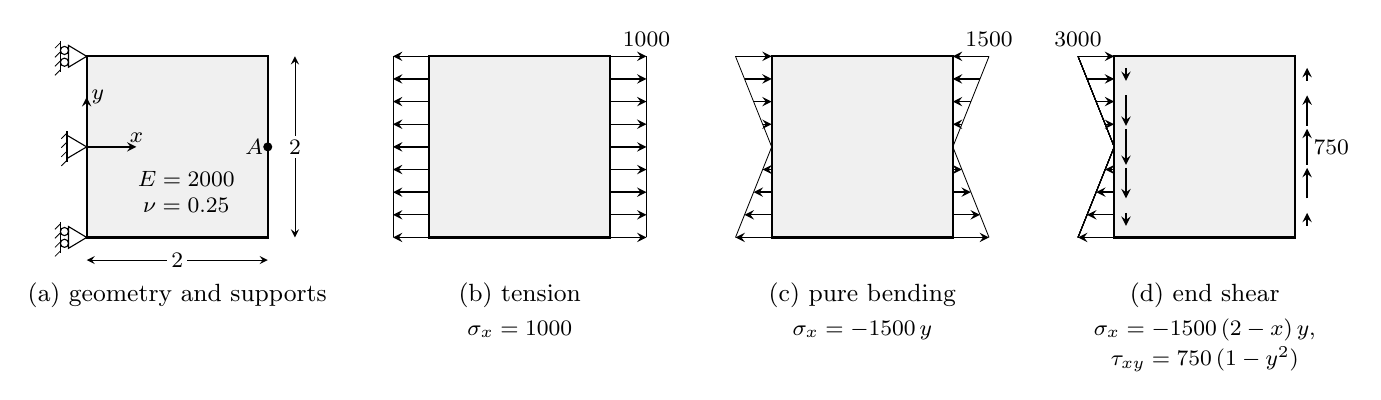
\begin{tikzpicture}[x=1.15cm, y=1.15cm,
    plabel/.style={anchor=north, font=\small, inner sep=0pt, align=center},
    slabel/.style={font=\footnotesize, inner sep=1.5pt},
    body/.style={draw=black, fill=gray!12, line width=0.8pt},
    trac/.style={-stealth, line width=0.5pt},
    roller/.pic={% apex at the node, restrains the displacement in the pic's x direction
      \draw[line width=0.4pt, fill=white] (0,0) -- (-0.2,0.12) -- (-0.2,-0.12) -- cycle;
      \draw[line width=0.4pt] (-0.245,0.065) circle (0.045) (-0.245,-0.065) circle (0.045);
      \draw[line width=0.6pt] (-0.29,0.17) -- (-0.29,-0.17);
      \foreach \s in {-0.15,-0.05,0.05,0.15} \draw[line width=0.3pt] (-0.29,\s) -- (-0.35,\s-0.06);},
    pin/.pic={% apex at the node, restrains both displacements
      \draw[line width=0.4pt, fill=white] (0,0) -- (-0.22,0.13) -- (-0.22,-0.13) -- cycle;
      \draw[line width=0.6pt] (-0.22,0.17) -- (-0.22,-0.17);
      \foreach \s in {-0.15,-0.05,0.05,0.15} \draw[line width=0.3pt] (-0.22,\s) -- (-0.28,\s-0.06);}]
% traction arrow at (#1,#2) on an edge with outward normal (#3,0), scaled
% traction (#4,#5): tail at the edge for tension, head at the edge for pressure
\def\panTrac#1#2#3#4#5{%
  \pgfmathsetmacro\pdn{(#4)*(#3)}%
  \pgfmathsetmacro\plen{veclen(#4,#5)}%
  \ifdim\plen pt>0.01pt
    \ifdim\pdn pt<0pt \draw[trac] ({#1-(#4)},{#2-(#5)}) -- (#1,#2);
    \else \draw[trac] (#1,#2) -- ++({#4},{#5});
    \fi
  \fi}
% (a) geometry and supports
\begin{scope}
  \draw[body] (0,-1) rectangle (2,1);
  \draw[-stealth, line width=0.5pt] (0,0) -- (0.55,0) node[slabel, above] {$x$};
  \draw[-stealth, line width=0.5pt] (0,0) -- (0,0.55) node[slabel, right] {$y$};
  \pic at (0,1) {roller};
  \pic at (0,-1) {roller};
  \pic at (0,0) {pin};
  \fill (2,0) circle (0.05) node[slabel, left] {$A$};
  \node[slabel, align=center] at (1.1,-0.5) {$E=2000$\\$\nu=0.25$};
  \draw[stealth-stealth, line width=0.3pt] (0,-1.25) -- node[slabel, fill=white] {$2$} (2,-1.25);
  \draw[stealth-stealth, line width=0.3pt] (2.3,-1) -- node[slabel, fill=white] {$2$} (2.3,1);
  \node[plabel] at (1,-1.5) {(a) geometry and supports};
\end{scope}
% (b) tension: sigma_x = 1000
\begin{scope}[xshift=4.35cm]
  \draw[body] (0,-1) rectangle (2,1);
  \foreach \y in {-1,-0.75,...,1} {
    \panTrac{2}{\y}{1}{0.4}{0}
    \panTrac{0}{\y}{-1}{-0.4}{0}}
  \draw[line width=0.3pt] (2.4,-1) -- (2.4,1) (-0.4,-1) -- (-0.4,1);
  \node[slabel, anchor=south, yshift=2pt] at (2.4,1) {$1000$};
  \node[plabel] at (1,-1.5) {(b) tension\\[1pt]\footnotesize $\sigma_x=1000$};
\end{scope}
% (c) pure bending: sigma_x = -1500 y (net moment 1000)
\begin{scope}[xshift=8.7cm]
  \draw[body] (0,-1) rectangle (2,1);
  \foreach \y in {-1,-0.75,...,1} {
    \panTrac{2}{\y}{1}{-0.4*\y}{0}
    \panTrac{0}{\y}{-1}{0.4*\y}{0}}
  \draw[line width=0.3pt] (2.4,-1) -- (2,0) -- (2.4,1) (-0.4,-1) -- (0,0) -- (-0.4,1);
  \node[slabel, anchor=south, yshift=2pt] at (2.4,1) {$1500$};
  \node[plabel] at (1,-1.5) {(c) pure bending\\[1pt]\footnotesize $\sigma_x=-1500\,y$};
\end{scope}
% (d) end shear: sigma_x = -1500 (2-x) y, tau_xy = 750 (1-y^2) (shear force 1000)
\begin{scope}[xshift=13.05cm]
  \draw[body] (0,-1) rectangle (2,1);
  % normal component on x = 0: t_x = 3000 y
  \foreach \y in {-1,-0.75,...,1}
    \panTrac{0}{\y}{-1}{0.4*\y}{0}
  \draw[line width=0.3pt] (-0.4,-1) -- (0,0) -- (-0.4,1);
  \node[slabel, anchor=south, yshift=2pt] at (-0.4,1) {$3000$};
  % shear component (own scale): t_y = 750 (1-y^2) on x = 2, -750 (1-y^2) on x = 0
  \foreach \y in {-0.8,-0.4,0,0.4,0.8} {
    \draw[trac] (2.13,{\y-0.2*(1-\y*\y)}) -- (2.13,{\y+0.2*(1-\y*\y)});
    \draw[trac] (0.13,{\y+0.2*(1-\y*\y)}) -- (0.13,{\y-0.2*(1-\y*\y)});}
  \node[slabel, right] at (2.15,0) {$750$};
  \node[plabel] at (1,-1.5) {(d) end shear\\[1pt]\footnotesize $\sigma_x=-1500\,(2-x)\,y$,\\\footnotesize $\tau_{xy}=750\,(1-y^2)$};
\end{scope}
\end{tikzpicture}\par\bigskip
\begin{tikzpicture}[plabel/.style={anchor=north, font=\small, inner sep=0pt}]
\begin{groupplot}[group style={group size=3 by 2, horizontal sep=0.9cm, vertical sep=0.85cm},
    hide axis, clip=false, x=2.45cm, y=2.45cm, xmin=0, xmax=2, ymin=-1, ymax=1,
    mesh/.style={black, line width=0.4pt},
    rot/.style={only marks, mark=*, mark size=1.4pt, black, samples at={0,90,180,270}},
    circ/.style={gray, dashed, line width=0.3pt, domain=0:360, samples=73}]
  \nextgroupplot
    \addplot[circ] ({1+0.5*cos(x)}, {0.5*sin(x)});
    \addplot[mesh] table {\data/panel_mesh_N1_t000.dat};
    \addplot[rot] ({1+0.5*cos(x)}, {0.5*sin(x)});
    \node[plabel] at (axis cs:1,-1.1) {(e) $\theta=0^\circ$};
  \nextgroupplot
    \addplot[circ] ({1+0.5*cos(x)}, {0.5*sin(x)});
    \addplot[mesh] table {\data/panel_mesh_N1_t090.dat};
    \addplot[rot] ({1+0.5*cos(x+90)}, {0.5*sin(x+90)});
    \node[plabel] at (axis cs:1,-1.1) {(f) $\theta=90^\circ$};
  \nextgroupplot
    \addplot[circ] ({1+0.5*cos(x)}, {0.5*sin(x)});
    \addplot[mesh] table {\data/panel_mesh_N1_t135.dat};
    \addplot[rot] ({1+0.5*cos(x+135)}, {0.5*sin(x+135)});
    \node[plabel] at (axis cs:1,-1.1) {(g) $\theta=135^\circ$};
  \nextgroupplot
    \addplot[circ] ({1+0.5*cos(x)}, {0.5*sin(x)});
    \addplot[mesh] table {\data/panel_mesh_N1_t175.dat};
    \addplot[rot] ({1+0.5*cos(x+175)}, {0.5*sin(x+175)});
    \node[plabel] at (axis cs:1,-1.1) {(h) $\theta=175^\circ$};
  \nextgroupplot
    \addplot[circ] ({1+0.5*cos(x)}, {0.5*sin(x)});
    \addplot[mesh] table {\data/panel_mesh_N1_t225.dat};
    \addplot[rot] ({1+0.5*cos(x+225)}, {0.5*sin(x+225)});
    \node[plabel] at (axis cs:1,-1.1) {(i) $\theta=225^\circ$};
  \nextgroupplot
    \addplot[circ] ({1+0.5*cos(x)}, {0.5*sin(x)});
    \addplot[mesh] table {\data/panel_mesh_N1_t270.dat};
    \addplot[rot] ({1+0.5*cos(x+270)}, {0.5*sin(x+270)});
    \node[plabel] at (axis cs:1,-1.1) {(j) $\theta=270^\circ$};
\end{groupplot}
\end{tikzpicture}
